\chapter{Introduction to Flexibility Management and The Goal of This Thesis}
\chaptermark{Introduction}
%http://www.tex.ac.uk/FAQ-runheadtoobig.html
\label{ch:introduction}

\section{Defining flexibility and flexibility management}
\sectionmark{Definitions}
Maintaining balance between supply and demand is a fundamental requirement to electric power system operations. The capability of a power system to match the supply and demand at each point of time by using controllable resources are often referred to as ``operational flexibility", or simply ``flexibility" \cite{Cochran2014,Wang2017,Lund2015,Delft}. Flexibility is therefore not a new concept. Power systems are inherently with uncertainty and variability since loads vary over time and occasionally in unexpected ways, and power plants may suffer unpredictable failures sometimes. All power systems are designed and built with certain level of flexibility to cope with those unexpected events. Conventionally, the flexibility is mainly enabled on the supply side, where dispatchable resources are controlled to adjust their outputs to match the time-varying load.

However, following radical transformation towards decarbonization, decentralization and digitalization in the energy industry, the existing operating model of electricity flexibility is being challenged and increasing interests are moving to flexibility from the load side and energy storage technologies\cite{Lund2015,Bronski2015,McKinsey&Company2010}. These disruptions are not only technological but also institutional and managerial, and are sparking market restructures and business model innovations. For instance, new flexibility resources are typically smaller in scale compared the traditional flexible generations so the new operating model is migrating to a more decentralized approach. Flexibility management, as an emerging business term, refers to the process how those new small-to-medium scale sources of flexibility are enabled, organized and exploited to serve the needs of less predictable power systems.

\section{Challenges in power system flexibility}
\sectionmark{Challenges}
The fundamental driver behind the increasing focus on power system flexibility is the global penetration of renewable energy sources (RES) such as wind and solar power \cite{Agency2016}. Many studies show that large-scale integration of RES brings critical challenges in maintaining power system balance with existing flexibility resources \cite{Cochran2014,Wang2017,Lund2015,FraunhoferIWES2015,Muller2016,Kwon2014,Kondziella2016,Papaefthymiou2016,Alizadeh2016,Bertsch2016}. 

The impact of RES on electric power systems can be deduced from the intrinsic technological attributes of RES \cite{Kondziella2016,Edenhofer2013}:
\begin{itemize}
	\item RES is variable and often viewed as non-dispatchable since its output is determined by weather conditions, and furthermore
	\item RES is often imperfectly predicted and specific power generation is uncertain until realization.
\end{itemize}

Effects of the property being non-dispatchable can be illustrated by introducing the concept of ``net load", also referred to as ``residual load", which equals the total system load minus the renewable generation and thus represents the load that needs to be served by non-RES resources \cite{Cochran2014,Muller2016,Ueckerdt2015}.

\begin{figure}[h!]
	\centering
	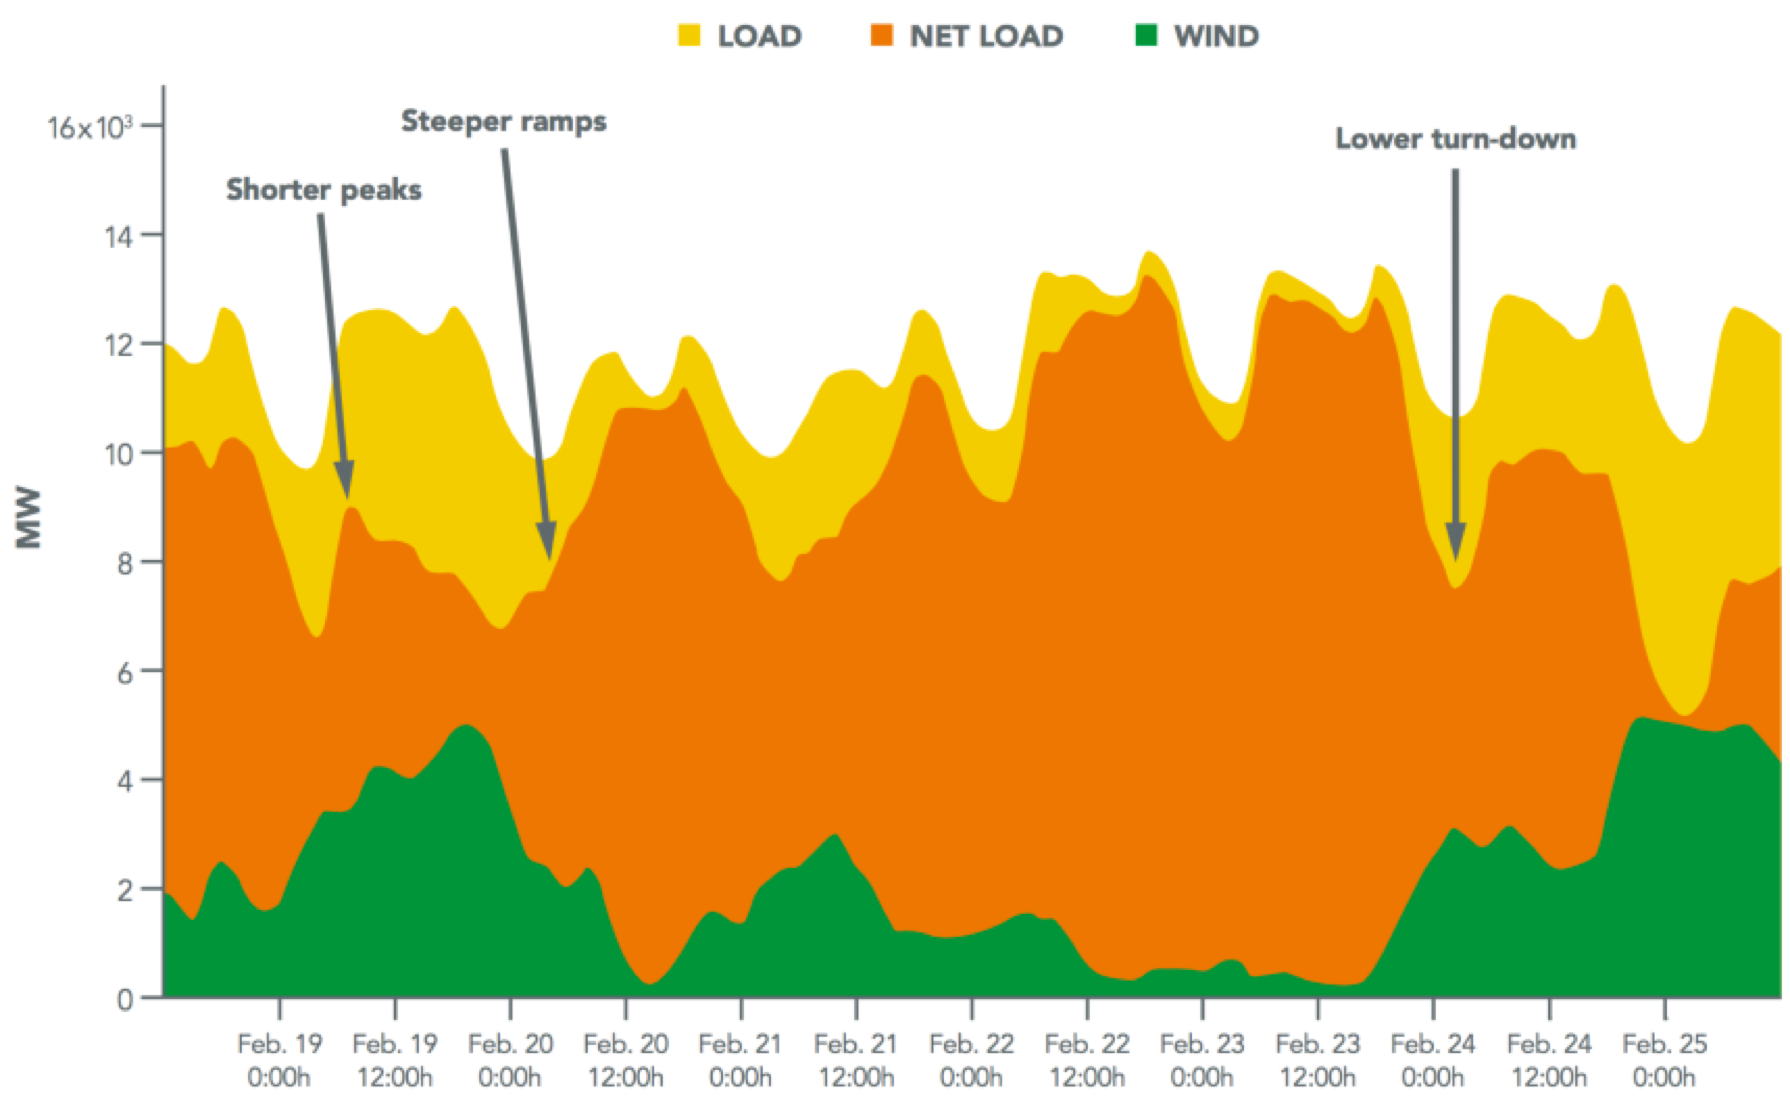
\includegraphics[width=0.9\linewidth]{Figures/NetLoad}
	\caption{An illustrative example of net load profile \cite{Cochran2014}}
	\label{fig:net-load}
\end{figure}

Figure \ref{fig:net-load} shows an example profile of net load, based on which we can see how RES is changing the profile of the existing non-RES generation:

\begin{itemize}
	\item \textbf{Shorter peaks}: resulting in fewer operating hours for conventional peak generators, affecting their cost recovery and consequently their ability to attract investors and maintain security security of supply
	\item \textbf{Lower turn-down}: diminishing the base load which should be stable at a higher level without RES, creating challenges to base generators who have limited operational flexibility to vary their outputs, and
	\item \textbf{Steeper ramps}: demanding higher performance in delivering flexibility, eliminating relatively low-grade resources from serving the needs for flexibility.
\end{itemize}

It can be seen that the whole span of the current generation portfolio serving base, flexible and peak power is under great pressure as a result of the RES growth.

The issue of the forecast error, on the other hand, requires the dispatch of flexibility close to real-time operation. This is an explicit issue in places where those activities are organized through power markets. In present power markets, the major part of the scheduling and pre-dispatching is determined ahead of the operating day based on forecasts and errors deviated in real time from the schedule are mostly depending on imbalance settlements via so-call frequency control ancillary services which are typically more costly\cite{Ranci2013,Srivastava2011}. The intra-day market with higher resolution of price signals and shorter prediction horizon toward actual operation is a feasible solution and implemented in many markets\cite{Srivastava2011} but intra-day markets are empirically prone to low liquidity in may regions \cite{Lund2015, Hagemann2015,Weber2010}. Without structural improvements in the market design, the demands for frequency control services would increase significantly and thus add burdens to the power system operators \cite{GEEnergyConsulting2014,Krad2017,Koch2009} as well as raise electricity prices for the end users. Measures such as improving day-ahead forecast \cite{Woo2016}, developing short-term frequency control products \cite{Gonzalez-Aparicio2015}, and optimized intra-day \cite{Weber2010} and balancing market frameworks \cite{Wartsila2014}, have been proposed. Being sensitively depending on the market arrangements, existing businesses may be disrupted significantly by any of those market restructures.

Besides, solar power which is forecasted to have even higher potential than wind power in the long run is tending to grow in distributed patterns \cite{Agency2016,Epia2016,Sawyer2016}. With the conventional centralized deployment of flexibility, local congestion is likely to worsen \cite{Lund2015,STEINKE2013826} which drives the needs for extensions of transmission and distribution capacity.

Collectively, RES penetration urges innovations in both technology and market design. Failing to do so would burden power system operators with higher expenses, potentially reducing the revenue scream of existing market players and/ or leading to significant curtailment of RES.

In addition to RES, the electrification of transportation, i.e. the penetration of plug-in electric vehicles (EV), is emerging more recently to be a second game changer. Facilitated by support policies from states and cities to uncap their multiple benefits such as transport decarbonization, air pollution reduction, and energy efficiency and security, the growth of EV has been accelerating significantly, having exceeded the global threshold of cumulatively 2 million in 2016 \cite{InternationalEnergyAgency2017}. Although a promising source of flexibility is the emergence of vehicle to grid (V2G) technologies \cite{Size2016,Habib2015,Foley2013}, barriers to its success are not trivial. The growth of EV may outpace developments in flexibility resulting in negative impacts such as increasing peak demand and potential local congestion \cite{Green2011,DBLP:journals/corr/PournarasJZFS17}.

It has been pointed out that the lack of flexibility can be identified more intuitively by signals such as \cite{Cochran2014,Wang2017}:
\begin{itemize}
	\item difficulty balancing demand and supply, resulting in frequency excursions or shedded load,
	\item significant renewable energy curtailments,
	\item negative market prices, and
	\item high price volatility in wholesale power markets.
\end{itemize}

Although having been discussed extensively for years in academia and by industry experts, it was not until quite recently when signs of inflexibility had been witnessed did the public start to be indeed aware of the challenges on power system flexibility. For instance, negative pricing in wholesale power spot market was first introduced in 2007 in Germany intra-day market and in 2008 in Germany/Austria day-ahead market\cite{EPEX_negative_price}, but real attention from the public came after 146 hours over 24 days were observed in the day-ahead market in 2017. Another famous example could be the power outage in South Australia that happened on September 28th 2016. After a widespread debate, Australia Energy Market Operator (AEMO) finally concluded in its investigation report that the generation deficit of wind farms due to unexpected operation of a control setting responding to multiple disturbances, led to the power blackout \cite{AEMO2016SA}.  This aroused public worries on supply security deriving from RES generation. As one of the follow-up actions, AEMO partnering with Tesla Inc., one of the leaders in global battery and electric vehicle markets,  built the worlds' largest battery energy storage system (BESS) in South Australia \cite{AEMO_tesla}.

These developments imply a proper timing for technology vendors to update their assessment on the market, as interests in flexibility management from the public and thus their potential customers have significantly increased.

\section{Technology options for system flexibility provision}
\sectionmark{Technologies}

Thanks to significant developments in energy storage technologies and information communication technologies (ICT) in recent years, the landscape of flexibility solutions has changed vastly. While it was in the past limited to centralized solutions, extracting flexibility from distributed resources and operating in an aggregate way has gradually become both technically feasible and economical viable \cite{Cochran2014,Wang2017,Lund2015,Muller2016}. A systematic summary for these various possibilities can be found as Figure \ref{fig:TechnologyOptions}.

\begin{figure}[h!]
	\centering
	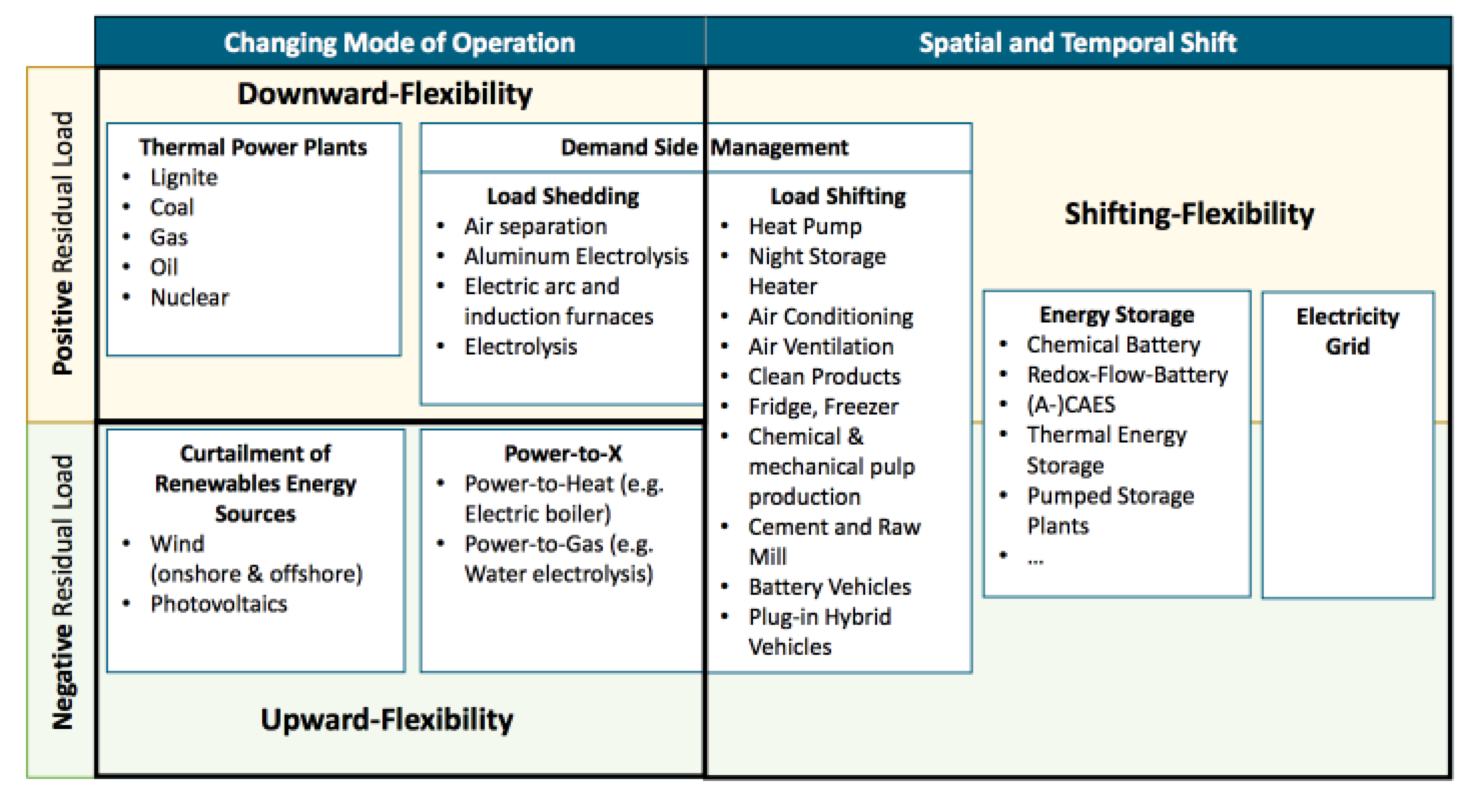
\includegraphics[width=0.95\linewidth]{Figures/TechnologyOptions}
	\caption{Catalog of flexibility solutions \cite{Muller2016}}
	\label{fig:TechnologyOptions}
\end{figure}

Technologies for flexibility are categorized by their type of provision:

\begin{itemize}
	\item \textbf{Downward-flexibility}: shedding demand or uplifting supply to reduce the positive residual load,
	\item \textbf{Upward-flexibility}: dropping surplus RES feed-in or increasing demand to mitigate negative residual load,
	\item  \textbf{Shifting-flexibility}: shuffling surplus energy from regions (or time steps) with negative or lower residual load to other regions (or time steps) with higher residual load.
\end{itemize}

It can be clearly seen that the term demand-side management (DSM), or often referred to as demand response (DR), is actually an umbrella term for a suite of different technologies with disparate flexibility mechanisms. 

Combining the evaluations carried out by several studies \cite{Cochran2014,Wang2017,Lund2015,Muller2016,Despres2017}, the characteristics of different technologies can be summarized on a high level as:

\begin{itemize}
	\item \textbf{Generation}: i.e. flexibility provision by varying power plant outputs. 
	
	This is by far the most mature technology and typically not constrained by the duration of flexibility provision nor how often to be activated. Activation time and ramp rate are the main issues for flexibility from power plants, especially conventional power plants using stream turbines, e.g. coal, lignite and nuclear power plants. Although output adjustments can be done within 1 hour, a cold start may take up to 100 hours or at least 4 hours even with the state-of-the-art thermal power plants \cite{Muller2016,AgoraEnergiewende2017}. Gas turbines are more flexible even compared to some other advanced technologies that are to be introduced later, so they are viable as a decent option to increase system flexibility \cite{Muller2016}.
	
	Cost is a complex topic and varies greatly between different type of generation technologies but in general flexible supply assets are still lower than most emerging flexibility technologies. However, building power plants is not an economical option to cover the extreme events that are rarely seen, as heavy fixed costs of building power plants are unlikely to be recovered in this scenario. Meanwhile, noxious emissions related to consumption of fossil fuels raise the uncertainty of operational viability in long term.
	
	\item \textbf{Load shedding}: i.e. load curtailment, mainly enabled by disrupting some energy-intensive industrial processes. In contrast to load shifting, shedded load will not be compensated later on as most of the time the industrial processes are running at their maximum allowances.
	
	Load shedding applications can provide fast responses, but are constrained at duration and numbers of activation. Nonetheless, short timespan of flexibility provision and limited occurrence fit the characteristics of extreme disturbances in power systems, so load shedding can be deployed for that specific purpose.
	
	The activation cost is essentially the loss caused by the disrupted productions so is indeed an adverse factor. The fixed cost, on the other hand, is less concerning as most industry plants nowadays are already equipped with automatic and intelligent energy management systems.
	
	\item \textbf{RES curtailment}: i.e. regulating the outputs of RES plants downwards.
	
	Technically, there are few constraints for RES curtailment as they can be performed promptly and frequently, and last for an indefinite time period. However, since curtailments will waive the revenues that would otherwise be received by selling electricity in the market, RES operators are discouraged to do so. Although a list of measures are possible for power system operators to mandate curtailments, it is contradictory to the overarching mandate of decarbonization. 
	
	Therefore, we deem the RES curtailment as a compromise and the last option if the needs for flexibility cannot be fulfilled by any other means.
	
	\item \textbf{Power-to-X(P2X)}: i.e. consuming excess electricity to produce other energy carriers, e.g. hydrogen, methane, heat, or other less conventional outputs.
	
	P2X technologies can also provide fast response and theoretically last for an indefinite period of time. However, in reality it is constrained by how the by-products are stored and utilized, and values of the by-products also vary significantly in different situations. For instance, while heat generation is valuable in winter, it is likely to be counterproductive in summer. 
	
	Regarding the cost, power-to-gas technologies require significant high initial investments on equipment while power-to-heat costs much less with the core components being boilers and heat tanks. Overall, the economics of P2X is still a challenging issue as the value can be harvested only if the by-products are competitive compared to goods by other production methods. However, production of P2X is destined to be intermittent as it would only be activated while upward-flexibility is needed reducing economic viability.
	
	\item \textbf{Energy storage}: a system that can absorb surplus energy in time with negative or low residual while release energy in time with higher demand. Due to its technical nature, the energy storage can act on both supply and demand side or be viewed as a third pillar of flexibility in conjunction with supply and demand \cite{Gunter2016}.
	
	Energy storage itself is an umbrella for an abundance of technologies, including battery energy storage systems (BESS), pumped hydroelectric storage (PHES), compressed air energy storage (CAES), flywheel, thermal storage, and others. These technologies vary significantly in their mechanism and thus in technical parameters such as size and efficiency as well as in performances, e.g. duration, action time, cost, etc. Among them, BESS could be the most attractive with fast response (activated within seconds), decent duration (up to 10 hours) and most importantly few external dependencies such as geographic topology. Cost is the main concern for batteries, but is decreasing dramatically in recent years \cite{Nykvist2015}; see Figure \ref{fig:BatteryFallingPrice}.
	
	\begin{figure} [h!]
		\centering
		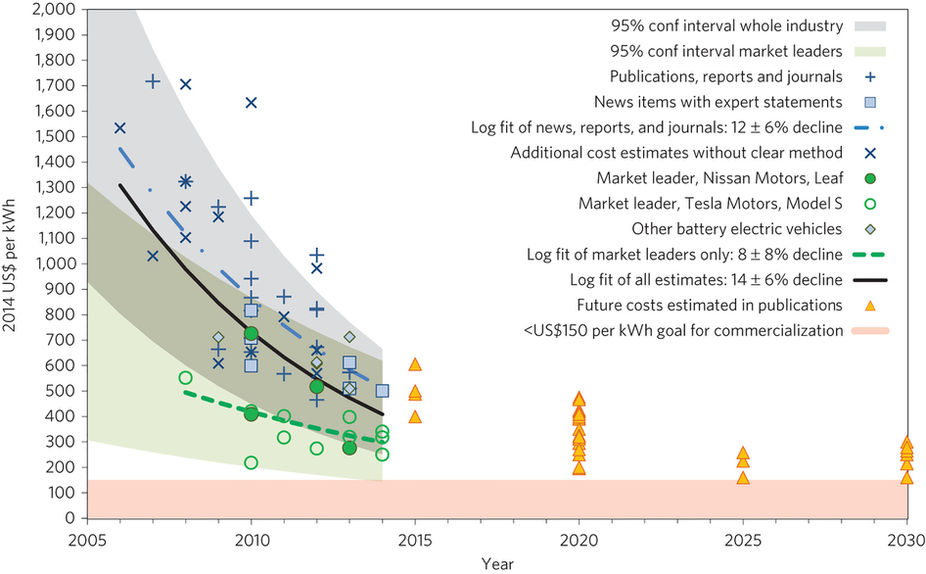
\includegraphics[width=0.95\linewidth]{Figures/BatteryFallingPrice.jpg}
		\caption{Cost of Li-ion batteries for electric vehicles \cite{Nykvist2015}.}
		\label{fig:BatteryFallingPrice}
	\end{figure}
	
	%\cite{Rastler2010,Eyer2010}
	
	%\begin{itemize}
		%\item \textbf{Batteries} use electrochemical reactions, i.e. oxidation-reduction processes between the battery's electrolyte and electrodes, converting electricity to chemical energy stored and vice verse. Battery is one of the most focused areas in research and an increasing number of novel batteries are being developed. More familiar and mature ones include lead-acid, lithium-ion, sodium/sulfur (Na/S), and others. Flow batteries, sometimes
		%\item \textbf{\item{}}
	%\end{itemize}
	
	\item \textbf{Load shifting}: corresponding to the concept of demand response in a narrower sense where responsive loads are enabled by direct control signals or indirect price signals.
	
	There are a great variety of load types that can be exploited for load shifting, so similar to energy storage, load shifting contains a list of subcategories. However, unlike other technologies that can be characterized by standard models, load shifting shows a higher diversity. This is because the characteristics of a load shifting system would be sensitively affected not only the technical parameters of load but also the control strategy and the users' preferences. Nonetheless, the load shifting in general has short activation time (within seconds to minutes), short duration (typically 0.5 to 8 hours) and relatively low cost (even close to zero if appliances come equipped with control devices). 

	\item \textbf{Electricity grid}: i.e. extension of distribution and transmission capacity. Distinguishing other technologies discussed above that shuffle electricity temporarily, the grid extension is the only option that deals with fluctuations of residual load spatially. %%%%%%
	%%%%%%%%%%%%%%%%%%%%%%%%%%%
	
	Flexibility from the transmission and distribution (T\&D) network has the fastest response and indefinite duration so together with generation flexibility it has been a main solution for conventional power system flexibility. However, challenges come from the development of distributed energy resources (DER) which disrupt the existing T\&D systems with altered electricity flow profiles. Congestion in the network is a major bottleneck for delivering flexible power in the grid. Further grid infrastructure upgrade may be necessary but leads to high expenses so may anyway need to be complemented by other technologies introduced above \cite{Cochran2014}.
	
\end{itemize}

Studies reveal that an abundance of different flexible technologies will be available in the future, and it is well agreed that no single option would be sufficient to individually provide flexibility to power systems \cite{Cochran2014,Wang2017,Lund2015,Muller2016}. Determining the best mix of options needs to be carried out on a case base and requires significant efforts as being a complex techno-economic and policy issue. 

The innovations in technology, changes in market frameworks and cost reductions will collectively change the landscape, and overall create more available solutions for players. Therefore, technology vendors are closely watching the development of technologies and constantly updating their view on which technologies to supply. 

\section{Applications, benefits and business models}
\sectionmark{Applications}
With the dual trends of both increasing level of RES penetration and growing opportunities from technological development, the necessity of increasing power system flexibility provision is being realized by policymakers, market designers, companies and the public. On the policy level, we have witnessed established rules that were based on the conventional technologies being constantly revisited and improved to better embrace new technologies. A good example is in the United States where the Federal Energy Regulatory Commission (FERC) has issued orders seeking the removal barriers and discrimination for emerging flexibility technology in markets organized by independent system operators (ISO) and regional transmission operators (RTO). Examples include Order No. 784 \cite{FERC784} published in 2013 calling for third-party flexibility provision in the ancillary service markets and Order No. 841 \cite{FERC841} published in 2018 opening gates for energy storage in wholesale energy markets. Similar efforts have been witnessed in Australia \cite{Brown2015,AEMO_DR}, South Korea and Japan\cite{Lipari2017}. European markets may lag behind in terms of implementation but active discussion and review on existing policies are being carried out \cite{ENTSO-E2015,EuropeanCommission2017,Poganietz2017}. Inspired by incentives from policies, innovative business models are being tested, for example the rise of aggregators and virtual power plants (VPP), a special case of aggregation with distributed generation being the core. 

Facing such a disruptive environment, it is a crucial task for technology vendors to update their understanding on the needs and use-cases of their utility customers in order to strategically plan their business and make decisions. The ask is understanding the applications and benefits of flexibility management.  Here ``application" refers to a use where flexibility is exploited for a certain aim via certain procedures, and ``benefit" denotes a value that can be evaluated in monetary or financial terms. Thereby the combination of players, applications, benefits and solutions constitute to a concrete business model.

More activities are observed in economies with liberalized power markets. This is not only because business innovations are inspired by competition in those markets and new entrants are allowed to bring more disruption, but also because of the fact that most of the major economies today have implemented or been in the process of power market liberalization \cite{Ranci2013,Vagliasindi2013}.

A schematic illustration of liberalized power markets can be found as Figure \ref{fig:PowerMarketSchematic}\footnote{In the figure, TSO is abbreviated for transmission system operator and DSO is for distribution system operator}.

\begin{figure}[h!]
	\centering
	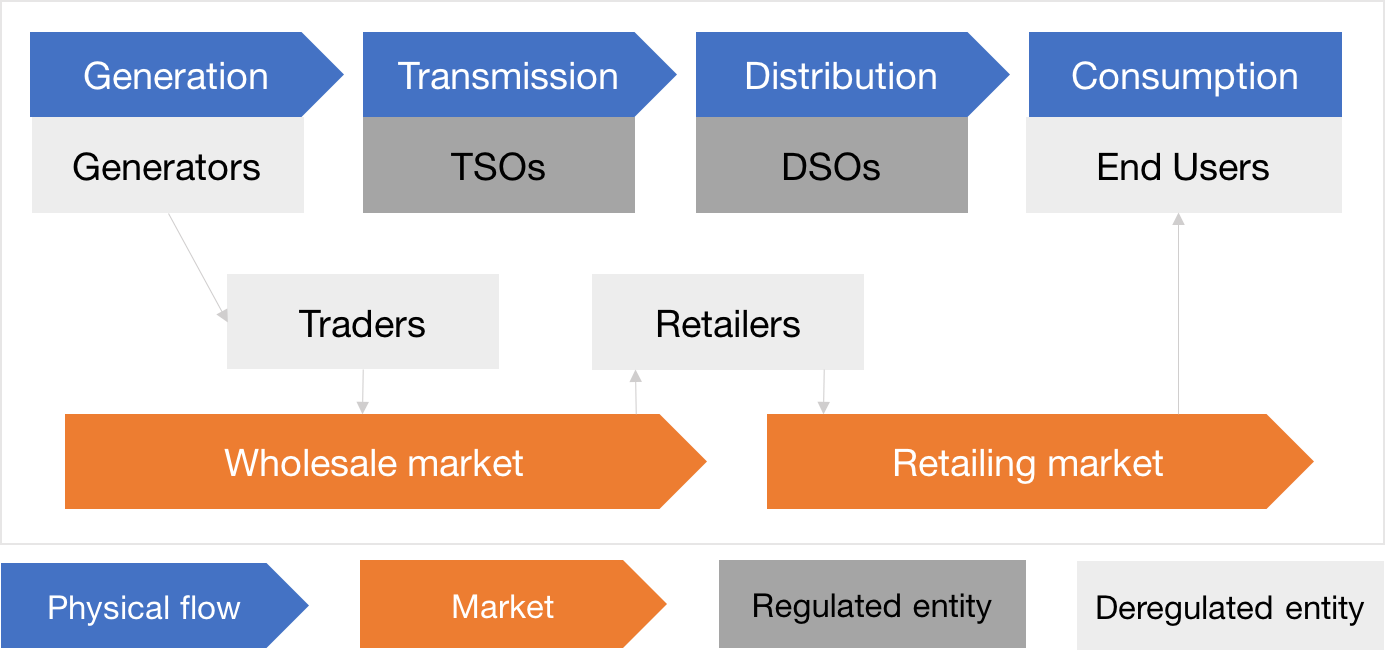
\includegraphics[width=0.95\linewidth]{Figures/PowerMarketSchematic}
	\caption{Schematic illustration of the liberalized power market}
	\label{fig:PowerMarketSchematic}
\end{figure}

Besides the conventional players shown in the chart, it is worthwhile to pay more attentions on the new role of aggregator. Aggregators are new entities in the electricity market that act as mediators / brokers for end-users to participate in wholesale markets \cite{He2011,Gkatzikis2013,Rahnama2014,HenriquezAuba2017,Lipari2017}. Unlike conventional retailers who are just responsible for one-way electricity sales to the consumers, aggregators enable two-way interaction with the end-users that make it possible for distributed energy resources (DERs) to be managed and utilized for a broader range of wholesale services. 
 
Varying from case to case, the wholesale electricity market is typically a bundle of different markets with distinct functions and possibly organized by various market operators. These functional markets include:

\begin{itemize}
	\item \textbf{Spot market}: also referred to as electricity market in a narrower sense, is the market where electricity is traded for immediate delivery. Typically, the spot electricity market is organized day-ahead but sometimes an intra-day or real-time market exists in some economies.
	\item \textbf{Financial derivatives market}: is a complement to the spot market. Electricity spot markets are typically highly volatile due to the physical nature of power systems. Financial derivatives, e.g. forwards, futures, swaps and options, are necessary tools in order to hedge the risk of trading in electricity market. They could be offered as standard exchange traded products in organized markets or via bilateral over-the-counter (OTC) contracts.
	\item \textbf{Ancillary service market}: is the market to supply services for the power system operators in order to maintain key technical characteristics of the system, including standards for frequency, voltage, network loading, and system restart processes.
	\item \textbf{Capacity market}: is a mechanism to pay capacity resources to be available to provide energy in order to ensure adequacy of electricity supply. The capacity is not always remunerated explicitly in some markets and those markets are therefore referred to as ``energy-only" markets \cite{Brown2015}.
\end{itemize}

Applications of flexibility management exist in all of these markets. Besides the financial derivative that is beyond the scope of focusing from a technology vendor's point of view, the major applications of flexibility the other markets are summarized as following:

\begin{itemize}
	\item \textbf{Electricity time-shift in wholesale spot market}: for shifting-flexibility technologies defined in the preceding section, they are able to shuffle electricity temporally so that can purchase inexpensive electricity that is available during periods when price is low and sell in high-pricing hours. The buying and selling activities can de done by real transactions in the wholesale market, or alternatively they can be realized by offsetting the players' position in the wholesale market. For instance, a player with a short position in the market may turn to flexibility resources for electricity output to offset the needs for purchasing and in this way the electricity can be conceived as sold by the flexibility resource while it does not necessarily involve a real transaction via wholesale market. It shall be noted that the electricity time-shifting in wholesale energy market is commonly referred to as ``\textbf{arbitrage}" by researchers on power system flexibility \cite{Walawalkar2007,Sioshansi2009,Connolly2011,Byrne2012,Bradbury2014,McConnell2015,Berrada2016,Zafirakis2016,Salles2017} and inherited by this thesis, but the term ``arbitrage" does not strictly fit in its finance-centric definition\footnote{In finance, arbitrage is defined as the simultaneous purchase and sale of identical or equivalent commodities or other instruments across two of more markets in order to benefit from a discrepancy in their price relationship, while arbitrage using flexibility does not always occur at the same time and is typically perform in only one market \cite{Eyer2010}.}
	
	\item \textbf{Electricity time-shift in retail market}: similar application of electricity time-shift can be realized in the retail market while the end-consumers are charged based on time-of-use tariffs. Conventionally, end-consumers do not have the capability of electricity generation and thus are not considered to inject electricity to the grid so the extraction of energy from flexibility resources is merely able to offset the users' needs. However, situations have altered with the penetration of distributed generations, mainly distributed RES, making the situation more close to the cases in wholesale markets. Nonetheless, the ability of consumers to benefit from this on an individual level is usually quite limited, which is why aggregators have moved in to make a liquid market.
	
	\item \textbf{Frequency control in ancillary services market}: frequency deviation is the most essential and immediate result of mismatching between supply and demand in power system. Recalling its definition, flexibility is without doubt most suited for providing frequency control services by quickly restore the divergences between generation and consumption. 
	
	\item \textbf{Supply capacity in capacity market}: as is introduced earlier, the capacity market is set up in some power markets to ensure supply adequacy. Flexibility that is able to shift the supply or shed the load can increase the resources adequacy on generation as well. Some capacity markets have admitted emerging flexibility technologies to receive remunerations, which is virtually a strong incentives to incorporate more flexibility in a power system.
	
	\item \textbf{Transmission congestion relief}: the transmission capacity has to keep pace with the peak demand. However, being disrupted by RES integration and EV penetration as we have discussed previously, the transmission system operators (TSOs) are under great pressure to upgrade infrastructure which is costly. Distributed flexibility enabled by emerging technologies, can be deployed at locations that are prone to variances in demand. By smoothing demand profiles and thus shaving the peaks in those areas, TSOs are relieved of congestion with lower transmission capacity and therefore cut expenses on transmission infrastructure.
	
\end{itemize}

Besides what is listed above, there are other applications that can be realized by certain type of flexibility technologies. For example, battery energy storage systems are normally able to provide voltage support and black start services \cite{Eyer2010,Rastler2010,Akhil2015}. However, these applications do not come from the ability of adjust supply and demand as we defined flexibility, so are excluded here.

Further to these applications, we need to understand the benefits that can be captured by users of flexibility. In this way, the benefit represents the willingness-to-pay (WTP) of the potential of of technology buyers, so can be an indicator to estimate the market potential for technology vendors. There two types of benefit:

\begin{itemize}
	\item \textbf{Variable income from power markets}: is the change in monetary receivables from power markets for players, which can be increased revenue or avoided losses that result from utilizing flexibility. This corresponds to deregulated players who are capable of participating in markets where flexibility has value as introduced earlier. These benefits can be calculated directly with power market data.
	\item \textbf{Deferred infrastructure expense}: match cases where players have certain obligations to fulfill. Emerging flexibility technologies can provide them solutions with reduced cost. This typically corresponds to the situation of regulated entities who are mandated to offer services with lowest possible cost. Their activities in power markets are sensitively controlled. The calculation for these benefits is less straightforward and requires comparison between proposed flexibility solutions to infrastructure investment. In non-liberalized markets benefits of vertically-integrated utilities can be categorized here.
\end{itemize}

Recalling the applications discussed earlier, apart from the transmission congestion relief where the benefits can be deemed as deferred expenses of TSOs, benefits of the other application can be all realized via power markets.

The potential business cases can be summarized on a high level as Table \ref{tab:summary-biz-model}.

\begin{table}[h!]
	\centering
	\begin{tabular}{L{2.5cm} L{2.5cm} L{2.5cm} L{2.5cm} L{3cm} }
		\hline
		\hline
		Application & Market & Benefit & Player & Solution \\
		\hline
		\hline
		Electricity time-shift & Wholesale spot market & Variable income & Generator, trader, retailer, aggregator & Temporal shifting-flexibility \\
		\hline
		Electricity time-shift & Retail market & Variable income\footnote{Here refers to reduced energy bills.} & Consumer & Temporal shifting-flexibility \\
		\hline
		Frequency control & Ancillary service market & Variable income\footnote{Both increased revenue by providing frequency control service and avoided losses due to obligated charges are possible depending on market specifications.} & Generator, retailer, aggregator & All options \\
		\hline
		Frequency control & Ancillary service market & Deferred expenses & TSO, DSO & All options \\
		\hline
		Supply capacity & Capacity market & Variable income & Generator, aggregator & Upward- and shifting- flexibility\\
		\hline
		Transmission congestion relief & - & Deferred expense & TSO, DSO & All options \\
		\hline
		\hline
	\end{tabular}
\caption{Summary of potential business models for flexibility management}\label{tab:summary-biz-model}
\end{table}

Finally, recalling our definition of flexibility management that is the process how those emerging flexibility solutions are enabled, organized and exploited to serve the needs of power systems, the role of technology vendors are clear in each of the cases listed above, which is:

\begin{itemize}
	\item Enabling flexibility - selling infrastructure (hardware) and technologies (software), and 
	\item Organizing flexibility and exploiting the benefits - providing consulting or managed services.
\end{itemize}

Certainly, depending on different market regimes and specific conditions, the business model and associated values could vary significantly, which is the essential rationale of carrying our this study.

%Visual power plant (VPP) is a special cases of aggregation that organizes micro-generators, loads and flexible storage capacities that are not necessarily geographically concentrated and participates in wholesale energy markets as a single power plant. Broadly speaking VPP is also a business model of flexibility management. Although the bulk energy sales as the main goal of VPP does not fit in the applications of flexibility, applications of arbitrage, providing frequency services and capacity availability are closely associated with it. 

\section{Research questions and scope}

Based on the observations introduced above, we perceive a promising business area. However, more concrete analysis both qualitatively and quantitatively would be necessary to support strategic decision making on flexibility management. Therefore, this thesis is designed to provide references for strategic decision making by answering the following questions:

\begin{itemize}
	\item What is the market value of flexibility
	\begin{itemize}
		\item in different markets?
		\item using different technologies?
	\end{itemize}
	\item How will this value change in scenarios with
	\begin{itemize}
		\item technological development - reduced costs?
		\item increased renewable penetration?
		\item other key factors?
	\end{itemize}
\end{itemize}

In order to answer these questions, we first map the landscape of flexibility management comprehensively and then conduct case-specific valuations of markets for flexibility management. A techno-economic model is established for the sake of quantitative analysis. It shall be noted that although some forward-looking analysis is included, the main purpose of this study is to offer a clear understanding of current situations and a framework that can be reused in the future to update this view.

%However, it shall be noticed this thesis is not intended to serve for:

%project developers to design a flexiblity system or make operating (including bidding) strategies of the system

%policy makers to redesign the electricity market structure, rules or other policies

%grid planners to understand the needs and options of flexibility in order to acheive system relability with lowest costs


Since flexibility management broadly covers a wide area of the technologies and economics of power systems, it is necessary to narrow the scope of this study to the selected topics.

\subsubsection{Scope of applications and benefits}

First of all, we focus only on deregulated players in liberalized power markets who can faster realize the benefits of technological disruption and innovation. The business cases related to regulated entities such as TSOs and DSOs are out of scope.

Secondly, this thesis focuses on applications in wholesale markets rather than retail markets as the end-consumers are not the primary customers for flexibility solutions. With respect to exploit action of distributed energy resources at the end-users' sites, we would only conceive the business cases involved with aggregators whose value realizations are also mainly in the wholesale markets.

Thereafter, what remains in our scope is: arbitrage in wholesale spot markets, providing frequency control in ancillary service markets and supply capacity in capacity markets. However, since capacity markets are not pervasive common practice in all regions, we will not include them in the core focus.

Finally, associated with the scoped applications, benefits are mainly variable incomes from power markets. In order to make it more clear, we further restrict the benefit being explicit monetary receivables from power markets, while all other associated benefits or by-products such as the societal goodness are excluded from consideration. 

\subsubsection{Scope of technology}

This thesis is focused on small-to-medium scale emerging flexibility solutions in low-to-medium voltage level, so flexibility provisions from conventional generation and pumped hydro energy storage (PHES) are excluded. Electricity grid extension also falls into this category, plus it is mainly of interests for TSOs who we have already excluded from our scope of applications.

Secondly, RES curtailment as is mentioned previously is considered as a compromise rather than opportunity. The benefits of RES curtailment may be valued from a system point view for grid stability maintenance. It will usually lead to no increase on explicit revenue for the players in power markets that is of our interests, unless the RES operators are obliged to meet the schedule and are punished for deviations.

P2X technologies are also excluded, because the values of its by-products such as hydrogen and heat are hard to account in a generic way and definitely not an explicit revenue from the power markets. Load shedding is out of scope for similar reasons, plus it is not an emerging technology with few growing opportunities for technology vendors.

Hence, we keep energy storage (excluding PHES) and demand response (load shifting) in our scope. It shall be noticed for qualitative analysis, it is normally not necessary to break them further up to sub-categories. e.g. thermal storage versus chemical storage, DR with air conditioning versus DR with heat pump , as the overall dynamics in terms of flexibility provision are generally unified. Furthermore, it is observed that in terms of policies and market rules they are seldom distinguished by technological sub-types \cite{FERC784,FERC841,PJMInterconnection2017}. However, when quantitative analysis is to be performed where technical performance and cost dynamics are to be studied, further distinction is unavoidable. In those cases, we have selected battery energy storage systems (BESSs) and electric vehicle to grid (EV2G) as two representatives of energy storage and load shifting respectively. 

\subsubsection{Scope of geographies}

Finally, for case studies, we scoped out three geographies with distinct power market regimes, i.e. PJM Interconnection in the United State, Germany, and New South Wales in Australia. The rationale is to select one geographic market from each of Americas, Europe and Asia-Pacific respectively.

\subsubsection{Outline of the thesis}

The remainder of this thesis is structured as follows: 

\begin{itemize}
	\item \textbf{Chapter 2} reviews the existing research works related to flexibility management, with a special focus on the quantitative valuation methodologies.
	\item \textbf{Chapter 3} maps the landscape of flexibility management by studying the market frameworks and the role of flexibility management in a generic way. Deeper analysis on value creations of flexibility management in different use-cases would be presented.
	\item \textbf{Chapter 4} introduces the methodology how the techno-economic model is established to make quantitative estimations.
	\item \textbf{Chapter 5} presents the results in three cases, i.e. PJM Interconnection, Germany and New South Wales. The case-specific business cases together with their quantified market potential and profitability would be provided, based on which we made analysis and recommendations for technology vendors.
	\item \textbf{Chapter 6} summarizes the main findings and conclusions. Outlook and recommended improvements by future works are also provided.
\end{itemize}
